\documentclass[10pt,doublespace]{article}
\usepackage{amsmath}
\usepackage{graphicx}
\usepackage{verbatim}
\usepackage{fancyhdr}
\usepackage[a4paper,margin=2.54cm]{geometry}
\pagestyle{empty}
\chead{\large \textbf{Mandeep Dhaliwal\\}}

\renewcommand{\headrulewidth}{0.8pt}

\begin{document}
\begin{center}
\large \textbf{Mandeep Dhaliwal\\}
\rule{\textwidth}{1pt}
\end{center}
{\bf \footnotesize
\noindent
Hostel 1, \hfill Contact:+91 6239098129 ~~~~~~~~~~~~~~\\
GNDEC,\hfill e-mailid: mandeepwt15@gmail.com\\
Ludhiana-141006,\\
Punjab
}

\begin{flushright}
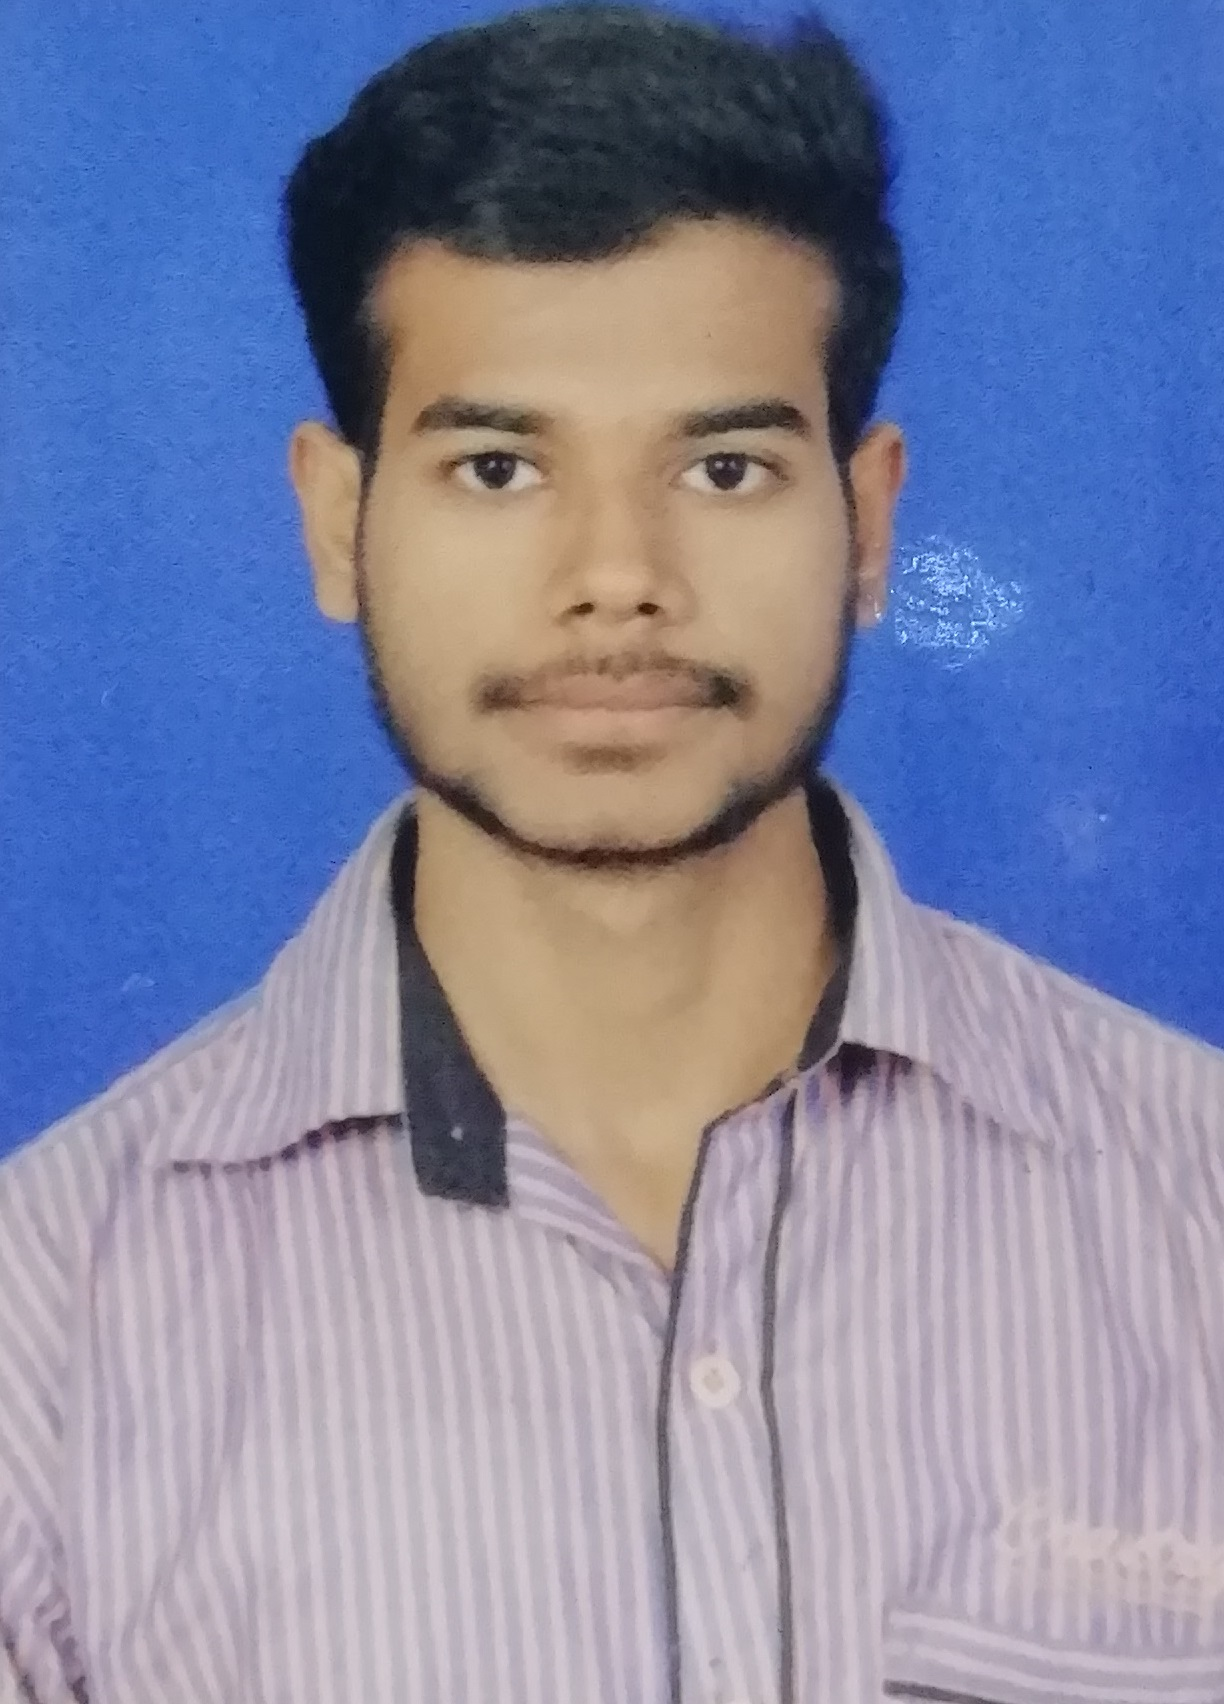
\includegraphics[scale=0.05]{me.jpg}
~~~~~~~~~~~~~~~~~~~~~~~~
\end{flushright}
 ~~ \\
\begin{tabular}{p{3cm}  p{10cm} }
 \begin{flushleft}\textbf{OBJECTIVE}\end{flushleft} &  \begin{flushleft}To implement new Technology and Solutions\end{flushleft}\\
\begin{flushleft} \textbf{EDUCATION}\end{flushleft}  &
\begin{flushleft}
\begin{tabular}{|p{2cm}|p{3cm}|p{3cm}|p{2cm}|p{2cm}|}

\hline
\bf Degree&\bf College/School&\bf University/Board&\bf Passing Year&\bf Pass percentage\\
\hline
X&Kendriya Vidyalaya &CBSE &2014 &9.0 CGPA\\
\hline
XII&Kendriya Vidyalaya &CBSE &2016 &90\% \\
\hline
B.Tech ECE&Guru Nanak Dev Engineering college, Ludhiana &Punjab Technical University &2020 (Ongoing) & - \\
\hline
\end{tabular}
\end{flushleft}\\
\begin{flushleft} \textbf{PROJECTS}\end{flushleft}&
\begin{enumerate}
\item Darkness Detector circuit using LDR
\item Square wave generator using op-amp
\item Automatic Fan Speed Controller
\item Electric vehicle speed controller
\item Program for Hospital Data Management
\item Program for Shortest Path Planning using Dijkstra's Algorithm
\item Machine Learning based Image Sorting on Raspberry Pi - NAS
\item Bot and Lift Mechanism for Nutty Squirrel Theme in eYRC 2018
\end{enumerate}\\
\begin{flushleft} \textbf{TRAINING \& INTERNSHIP}\end{flushleft}&
\begin{itemize}
\item 6 weeks Training at NIELIT, Chandigarh in RaspberryPi with Python
\item Internship as Campus Ambassador in Internshala Student Program 8.0
\end{itemize}\\
\end{tabular}\\
\begin{tabular}{p{3cm}  p{10cm} }
\begin{flushleft} \textbf{RESEARCH PUBLICATIONS}\end{flushleft}&\begin{flushleft} None \end{flushleft}\\
\begin{flushleft} \textbf{TECHNICAL SKILLS}\end{flushleft}&
\begin{itemize}
\item C and C++
\item Python
\item \LaTeX
\item Assembly for 8085 microprocessor and 8051 microcontroller
\item AVR C (ATmega2560)
\item Embedded Systems
\end{itemize}\\
\begin{flushleft} \textbf{SOFT SKILLS}\end{flushleft}&
\begin{enumerate}
\item Management
\item Self Motivation
\item Leadership and Teamwork
\item Flexibility
\end{enumerate}\\
\begin{flushleft} \textbf{EXTRA-CURRICULAR ACTIVITIES}\end{flushleft}&
\begin{itemize}
\item Member of Organising Team in Atharva 2018 at GNDEC
\item National Service Scheme volunteer
\item Sports
\item Participation in various events at college level
\end{itemize}\\
\begin{flushleft} \textbf{CO-CURRICULAR ACTIVITIES}\end{flushleft}&
\begin{enumerate}
\item Member of SAE INDIA (2018-19)
\item Member of Computer Society of India, GNDEC (2018-present)
\item Team member in Team Reventon for Efficycle 2018 Competition by SAE at LPU, Phagwara, Team Secured 12th position all over India 
\item Team Leader in Team for eYantra Robotics Competetion at IIT Bombay, Team Id 1990 secured 5th Position at Finals
\item 4th position in Workshop on Python for Data Science by CSI, GNDEC
\end{enumerate}\\
\begin{flushleft} \textbf{Personal Details}\end{flushleft}&
\begin{flushleft} \textbf{Father’s Name:} Nahar Singh\newline \textbf{Mother’s Name:} Prem Lata\newline \textbf{Sex:} Male\newline \textbf{Date of Birth:} 4 Feb 1999\newline \textbf{Nationality:} Indian\newline \textbf{Marital Status:} Single
\end{flushleft}\\
\end{tabular}\\
\begin{tabular}{p{3cm}  p{10cm} }
\begin{flushleft} \textbf{Reference}\end{flushleft}&
\begin{flushleft} None
\end{flushleft}\\
\begin{flushleft} \textbf{Declaration}\end{flushleft}&
\begin{flushleft} All the details provided by me are correct to my Knowledge
\end{flushleft}\\
 \end{tabular}


\end{document}